\section{Implementation}\label{sec:implementation}
% How Fault Tolerance mechanisms are implemented
This section will cover the implementation of the fault-tolerance mechanisms
covered in Section~\ref{sec:mechanisms} on the architecture described in
Section~\ref{sec:architecture}.

\subsection{Timeouts}
Implementing HTTP requests in Python is straightforward using the
\textit{requests}
library\footnote{http://docs.python-requests.org/en/master/} as shown
in Listing~\ref{lst:requestnotimeout}.

\begin{lstlisting} [
	language=python,
	caption={GET request from the trader service to the account
          service without timeout.},
	breaklines=true,
	label={lst:requestnotimeout}]
requests.get("http://account:5001/account/" + str(accountId))
\end{lstlisting}
In the example architecture all requests from the
trader service to the account service and all requests from the trader
service to the stock service must include timeouts. Neither the
account service nor the stock service has any outgoing requests, so no
timeouts are implemented here.
\\\\
It is desirable to use the same timeout value for requests to the same
service, so these are extracted into a configuration variable. Adding
timeouts simply requires an additional argument to the request with
the desired timeout resulting in requests on the form as seen in
Listing~\ref{lst:requesttimeout}.

\begin{lstlisting} [
	language=python,
	caption={GET request from the trader service to the account
          service with timeout. The variable \textit{account\_timeout}
          holds a float denoting the number of seconds before the
          request times out.},
	breaklines=true,
	label={lst:requesttimeout}]
requests.get("http://account:5001/account/" + str(accountId),
             timeout=account_timeout))
\end{lstlisting}

\subsection{Bulkheads}
The purpose of implementing bulkheds is to limit the number of
concurrent requests from one service to another. Using semaphores is a
clear way to accomplish this. In this implementation bounded
semaphores from the Python threading
module\footnote{https://docs.python.org/2/library/threading.html} is
used.
\\\\
One semaphore must be created for each resource, so in the case of the
trader service two semaphores are created - one for requests to the
account service and one for requests to the stock service. The
semaphore setup is listed in Listing~\ref{lst:semaphoresetup}.

\begin{lstlisting} [
	language=python,
	caption={Initialising semaphores to be used in the trader
          service. \textit{account\_sema} is the semaphore used to
          limit access to requests to the account service and
          \textit{stock\_sema} is the semaphore used to limit access
          to requests to the stock service. Each semaphore is
          initalised in this example to accept a maximum of 100
          concurrent requests.},
	breaklines=true,
	label={lst:semaphoresetup}]
account_max_connections = 100
stock_max_connections = 100
account_sema = threading.BoundedSemaphore(value=account_max_connections)
stock_sema = threading.BoundedSemaphore(value=stock_max_connections)
\end{lstlisting}
For the bulkheads to function correctly the account semaphore must
always be acquired before making a request to the account service and
accordingly for requests to the stock service as displayed in
Listing~\ref{lst:semaphoreuse}. In the case of full capacity load
where the maximum number of allowed concurrent requests are active,
the semaphore cannot be acquired. This results in an error being
thrown and the request is rejected. For the trader service this means
that the requested trade is refused, but this now happens instantly
with no risk of the request hanging. No more requests are accepted
before the semaphore is released one or more times.

\begin{lstlisting} [
	language=python,
	caption={Acquiring the account semaphore and making a request
          to the account service if successful. If the semaphore
          cannot be acquired an error is raised and the request is
          rejected.},
	breaklines=true,
	label={lst:semaphoreuse}]
sema = account_sema.acquire(false)
if sema:
  requests.get("http://account:5001/account/" + str(accountId),
             timeout=request_timeout))
  account_sema.release()
else:
  # no threads available - throwing error!
  ...
\end{lstlisting}

\subsection{Circuit Breaker}
The circuit breaker has been implemented as a state-machine, with the
circuits state being stored in a local variable and events being functions.
Calls are executed by the circuit breakers \texttt{call(func)} function, which takes
an anonymous function, executes it, monitors for failures, returns result if
successful, tries again if not and raises \texttt{CircuitOpenError} if number of
failures reach defined max. The implementation of \texttt{call(func)} can be found in
Listing~\ref{lst:circuitbreakercall} and an example of invocation can be found
in Listing~\ref{lst:circuitbreakerinvocation}.
\\\\
The circuit breakers maximum number of failures, \texttt{fail\_max}, and the duration
of its reset timeout, \texttt{reset\_timeout}, can be configured. These can be used for
fine-tuning the circuit breaker to the service it is associated with. 
\\\\
This implementation of a circuit breaker is very simple, since it only acts on
the function it is handed. If the function raises an error/exception it is
interpreted as a failure and if it executes as expected, it interprets it as a
success. Alternative approaches could be to fail on exhaustion of thread pool
or overflowing message queues.
\\\\
The system utilizes the circuit breaker only in the \textit{trader} service,
from the \textit{trader} service to both \textit{account} service and 
\textit{stock} service, resulting in two circuit breakers, one circuit breaker
per service dependency. Circuit breaker states are local to instances of the 
\textit{trader}.

\begin{lstlisting} [
	language=python,
	caption={Example of invocation of the circuit breaker \texttt{call} function, from
		the \textit{trader} service to the \textit{account} service. The anonymous
			function is wrapped in a Python \texttt{lambda} expression.},
	breaklines=true,
	label={lst:circuitbreakerinvocation}]
res = account_circuit.call(
		lambda: requests.get("http://account:5001/account/" + str(accountId),
			timeout=request_timeout))
\end{lstlisting}

\begin{lstlisting} [
	language=python,
	caption={The implemented \textit{Circuit Breakers} wrapper function, named
		\texttt{call}. The function takes an anonymous function (in python a \texttt{lambda}
				expression), invokes it if the circuit is closed and generates the
			events which will trigger a state change according to the state machine
			described in Figure~\ref{fig:circuitbreakerstate}. The anonymous function
			will be called repeatedly until it either succeeds or reaches the defined
			maximum of failures and opens the circuit. If the circuit is
			open, the anonymous function will not be invoked, but the circuit will
			fail quickly instead, unless the reset-timeout has been reached which
			will allow the function to be called in order to test if the called
			service is functioning as expected again.},
	breaklines=true,
	label={lst:circuitbreakercall}]
def call(self, func):
	# Closed Circuit
	if self.state == self.CLOSED:
		try:
			res = func()
			self.success()
		except:
			self.log("Unexpected error:", sys.exc_info()[0])
			self.fail()
			if self.state == self.CLOSED:
				res = self.call(func) # Calling again
			else:
				self.reset_timer_start = dt.datetime.now()
				raise CircuitOpenError()
							
	# Open Circuit
	elif self.state == self.OPEN:
		self.log("Reset time is at: " + str((dt.datetime.now() -
			self.reset_timer_start).total_seconds()))
		if self.reset_timeout <= (dt.datetime.now()
					- self.reset_timer_start).total_seconds():
			try:
				self.reset()
				res = func()
				self.success()
			except:
				self.fail()
				self.reset_timer_start = dt.datetime.now()
				raise CircuitOpenError()
		else:
			raise CircuitOpenError()

	# Half-Open Circuit
	elif self.state == self.HALFOPEN:
		try:
			res = func()
			self.success()
		except:
			self.fail()
			self.reset_timer_start = dt.datetime.now()
			raise CircuitOpenError()
	return res
\end{lstlisting}

\subsection{Containers}
Each of the three microservices are implemented to run within \textit{Linux
Containers}, utilizing the \textit{Docker} platform. They all run within the
same \textit{Docker image}, specified in the \textit{Dockerfile} found in
Listing~\ref{lst:dockerfile} and on \textit{Docker Hub} under the name
\textit{sthordall/microtrader}~\cite{microtraderimage}. The images extends the
official \textit{python:2.7.12} image and exposes the needed ports, adds the
source code, builds it and accepts a command to start the wanted service.
\\\\
A service is started with the \textit{Docker} orchestration tooling, and the
whole system can be brought up with the script found in
Listing~\ref{lst:startallservices}. The script results in the architecture
shown in Figure~\ref{fig:containerarchitecture}. A reverse proxy based on
\textit{NGINX} has been setup to forward requests to the services, allowing for
a single point of invocation.

\begin{lstlisting} [
	language=docker,
	caption={Dockerfile defining Linux container image, which all three services
		run within.},
	breaklines=true,
	label={lst:dockerfile}]
FROM python:2.7.12

EXPOSE 5001 5002 5003

ADD . /service
WORKDIR /service

RUN python setup.py install
\end{lstlisting}


\begin{lstlisting} [
	language=bash,
	caption={Script for starting microservice architecture in the linux container
	orchestration tool \textit{Docker Swarm}. The resulting architecture consists
	of the three services, \texttt{trader}, \texttt{stocks} and \texttt{account}, their associated
	databases \texttt{stocks-db} and \texttt{account-db}. Furthermore a reverse proxy has been
	setup to forward requests to the three services, \texttt{proxy}, allowing for a 
	single point of invocation. All three services are started with no
	replication, i.e.\ a single instance per service, but are ready to be scaled,
	utilizing \textit{DNS Round Robin} load balancing. All services interact
		through the virtual network called \texttt{swarm\_net}, and the \texttt{proxy} exposes port
	80 to external network.},
	breaklines=true,
	label={lst:startallservices}]
#!/bin/bash
# Trader service
docker service create \
	--network swarm_net \
	--name trader \
	--endpoint-mode dnsrr \
	--replicas 1 \
	sthordall/microtrader:latest \
	python services/trader.py

# Stocks service
docker service create \
	--network swarm_net \
	--name stocks \
	--endpoint-mode dnsrr \
	--replicas 1 \
	sthordall/microtrader:latest \
	python services/stocks.py

# Stocks-DB
docker service create \
	--network swarm_net \
	--name stocks-db \
	--replicas 1 \
	redis:latest

# Account service
docker service create \
	--network swarm_net \
	--name account \
	--endpoint-mode dnsrr \
	--replicas 1 \
	sthordall/microtrader:latest \
	python services/account.py

# Account-DB
docker service create \
	--network swarm_net \
	--name account-db \
	--replicas 1 \
	redis:latest

# NGINX Proxy
docker service create \
	--network swarm_net \
	--name proxy \
	--replicas 1 \
	--publish 80:80 \
	sthordall/traderproxy:latest
\end{lstlisting}

\begin{figure}[H]
\centering
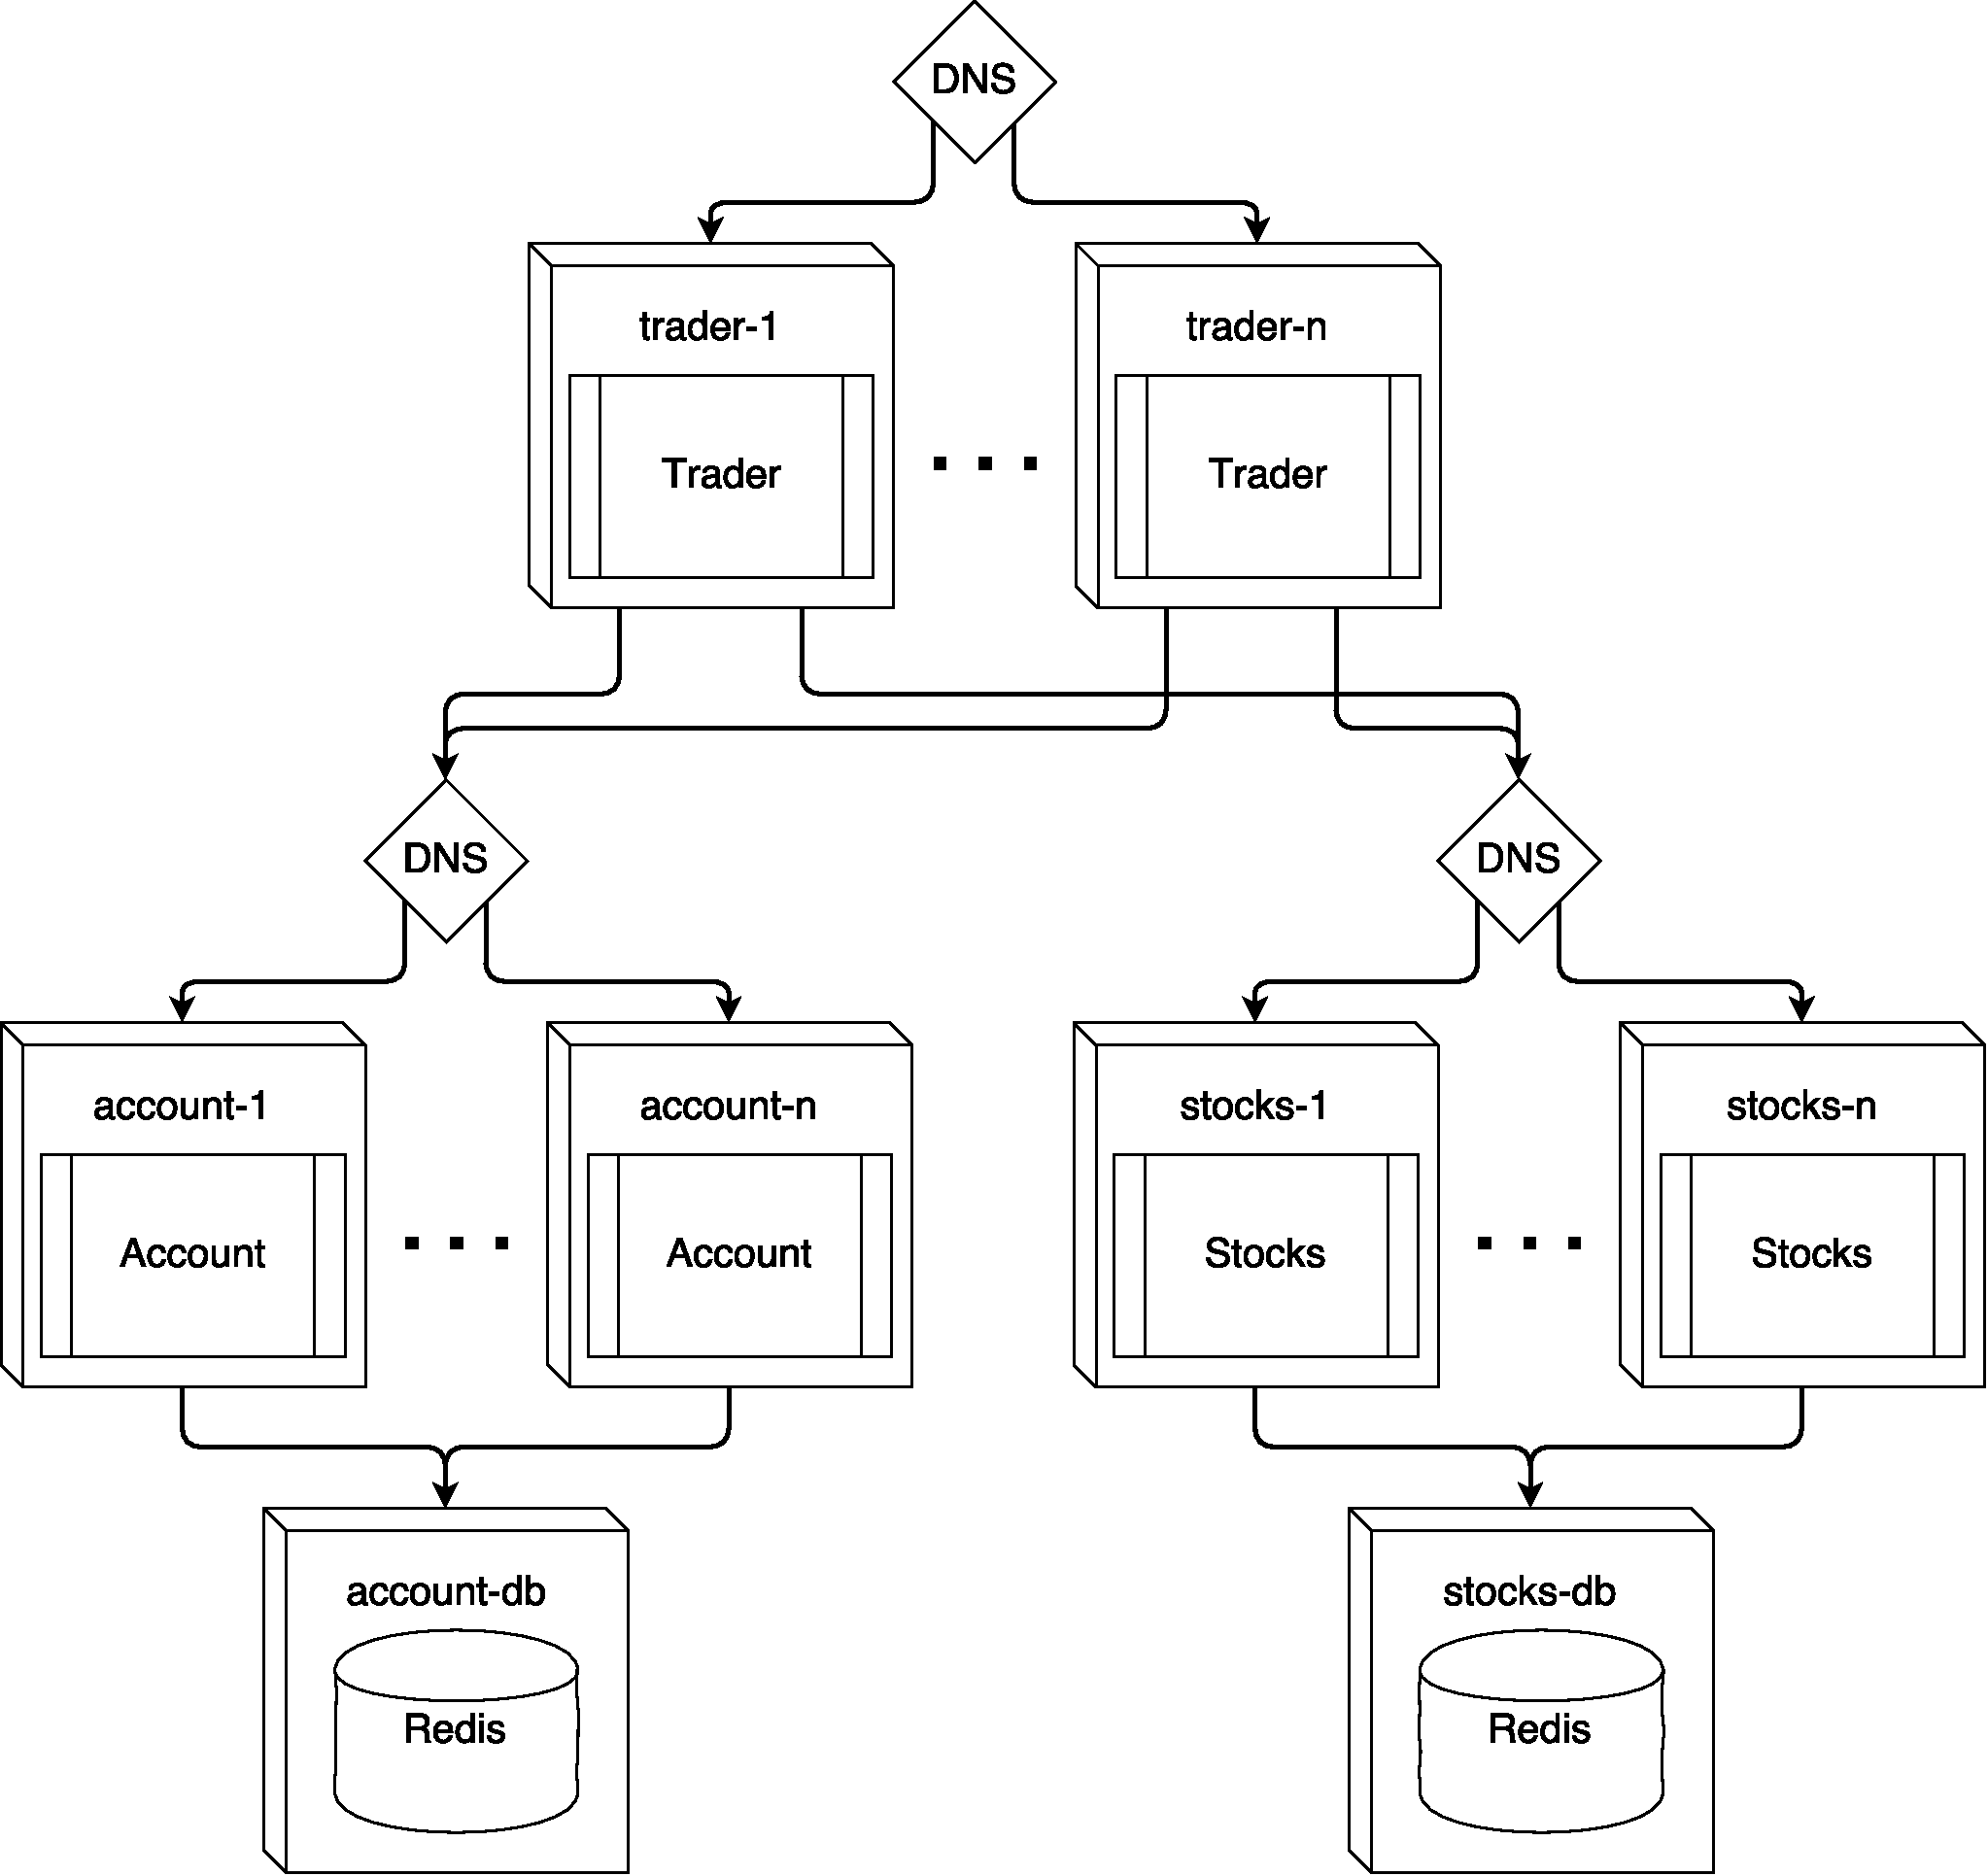
\includegraphics[width=0.7\textwidth]{../media/container_architecture.pdf} 
\caption{The resulting architecture from running script in
	Listing~\ref{lst:startallservices}. The proxy forwards requests to the three
		services, which can be replicated to $n$ instances. Load balancing is done
		with \textit{DNS Round Robin}. Databases and proxy are not expected to
		replicate.}
\label{fig:containerarchitecture}
\end{figure}

\subsection{Replication}
Replication has been implemented by utilizing the Linux container orchestration
and clustering tooling in \textit{Docker}. \textit{Docker} manages the
services, or rather the containers they run within, across a cluster created
with \textit{Docker Swarm}. It handles domain names, load balancing, restarting
of failed services and virtual networking. The cluster used for testing
consists of 4 nodes, 2 acting as managers and 2 acting as workers. 
\\\\
When the services have been started with the script from 
Listing~\ref{lst:startallservices}, they can be seen running spread across the
cluster, with the command \texttt{docker service ps <service-name>}, example of the
output can be seen in Figure~\ref{fig:serviceps}. Replication can either be
defined as part of the \texttt{--replicas} option when starting a service, see
Listing~\ref{lst:startallservices}, or after the fact with the \texttt{docker service scale
SERVICE=REPLICAS}. Service replicas are spread across the cluster, see
Figure~\ref{fig:serviceps}, with \textit{Docker} trying to spread each service to as
many nodes as possible.
\\\\
Load is balanced across the replicas, by use of \textit{DNS Round Robin}, which
translates DNS requests to differing host IPs, e.g.\ for each request to host
\texttt{account} the host-name is translated to a different replica.

\begin{figure}[H]
\centering
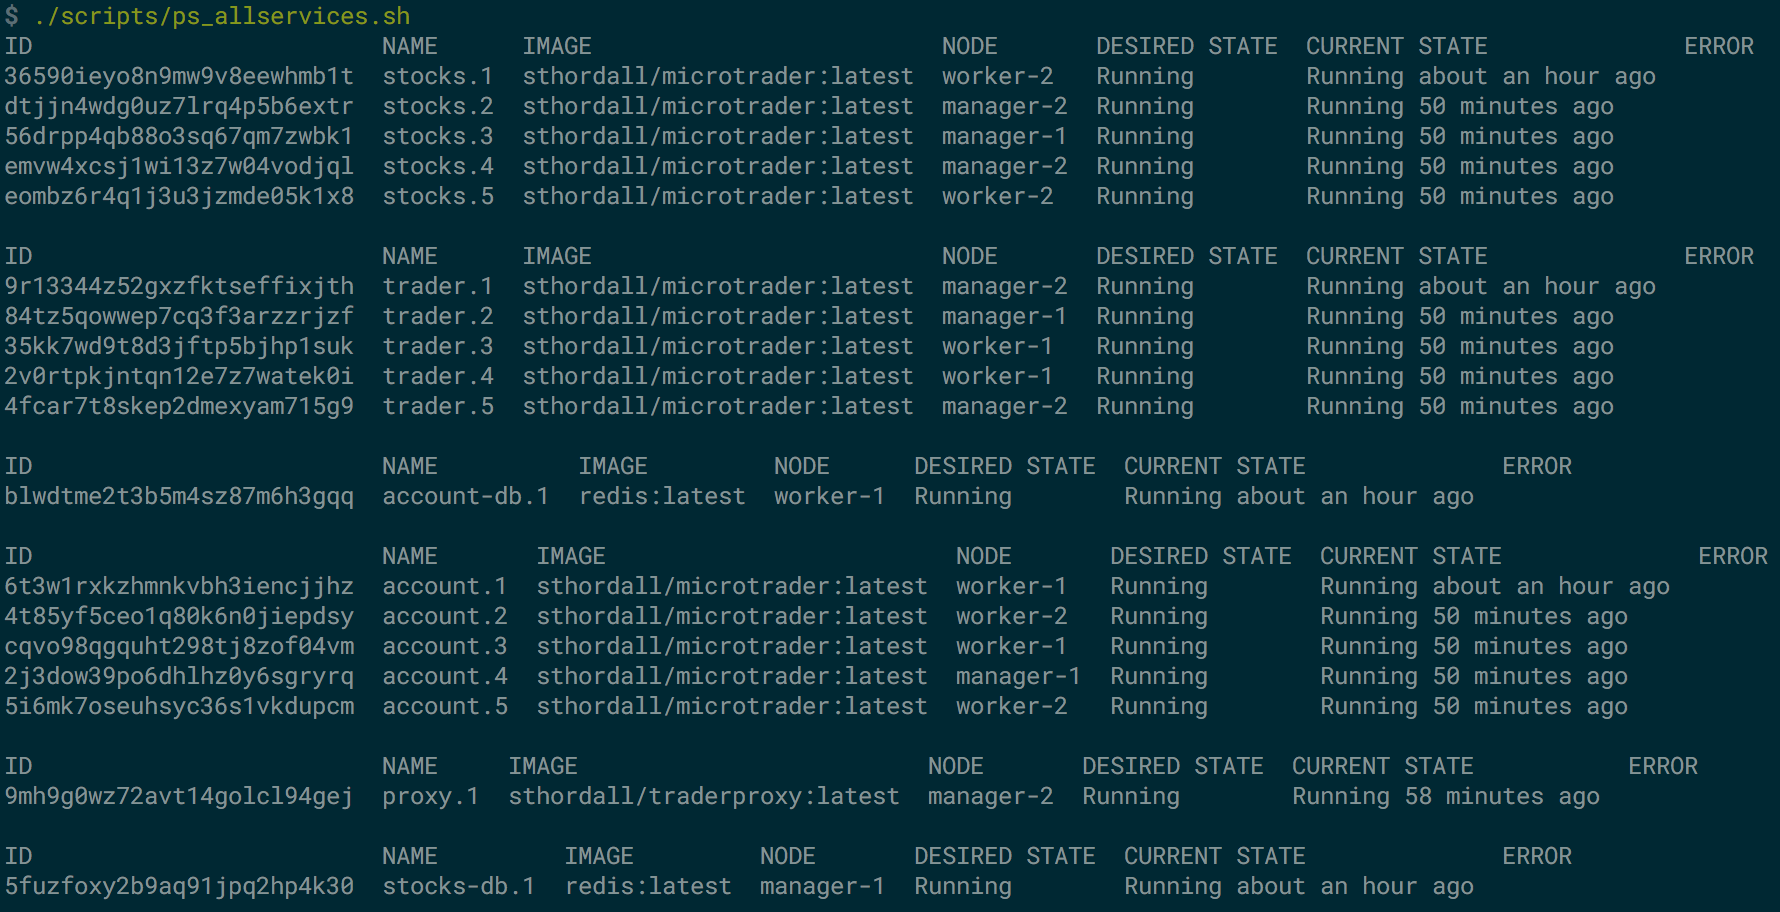
\includegraphics[width=\textwidth]{../media/serviceps.png} 
\caption{Output from \texttt{docker service ps <service-name>} on all services
	in cluster. The \texttt{trader}, \texttt{account} and \texttt{stock} services
  have been scaled to 5 replicas, which are spread so each service runs on as
	many nodes as possible.}
\label{fig:serviceps}
\end{figure}

\subsection{Redundancy}
Redundancy has mainly been implemented using clustering with \textit{Docker Swarm}
and \textit{Active/Active} failover in the form of replication. The cluster
consists of 4 virtual machines, each running \textit{Docker Engine}, with 2
assigned as \textit{managers} and 2 assigned as \textit{workers}.
A manager node handles the orchestration of services across the cluster,
ensuring that the services run in the defined number of replicas and that if a
node goes down, its services are transferred to another node. A demonstration
of this can be seen in Figure~\ref{fig:servicefailover}
\\\\
This system has a single redundant manager \texttt{manager\_2}, which runs in
\textit{Active/Passive} failover, ready to take over as manager should 
\texttt{manager\_1} die, as demonstrated in Figure~\ref{fig:manager1leader}.

\begin{figure}[H]
\centering
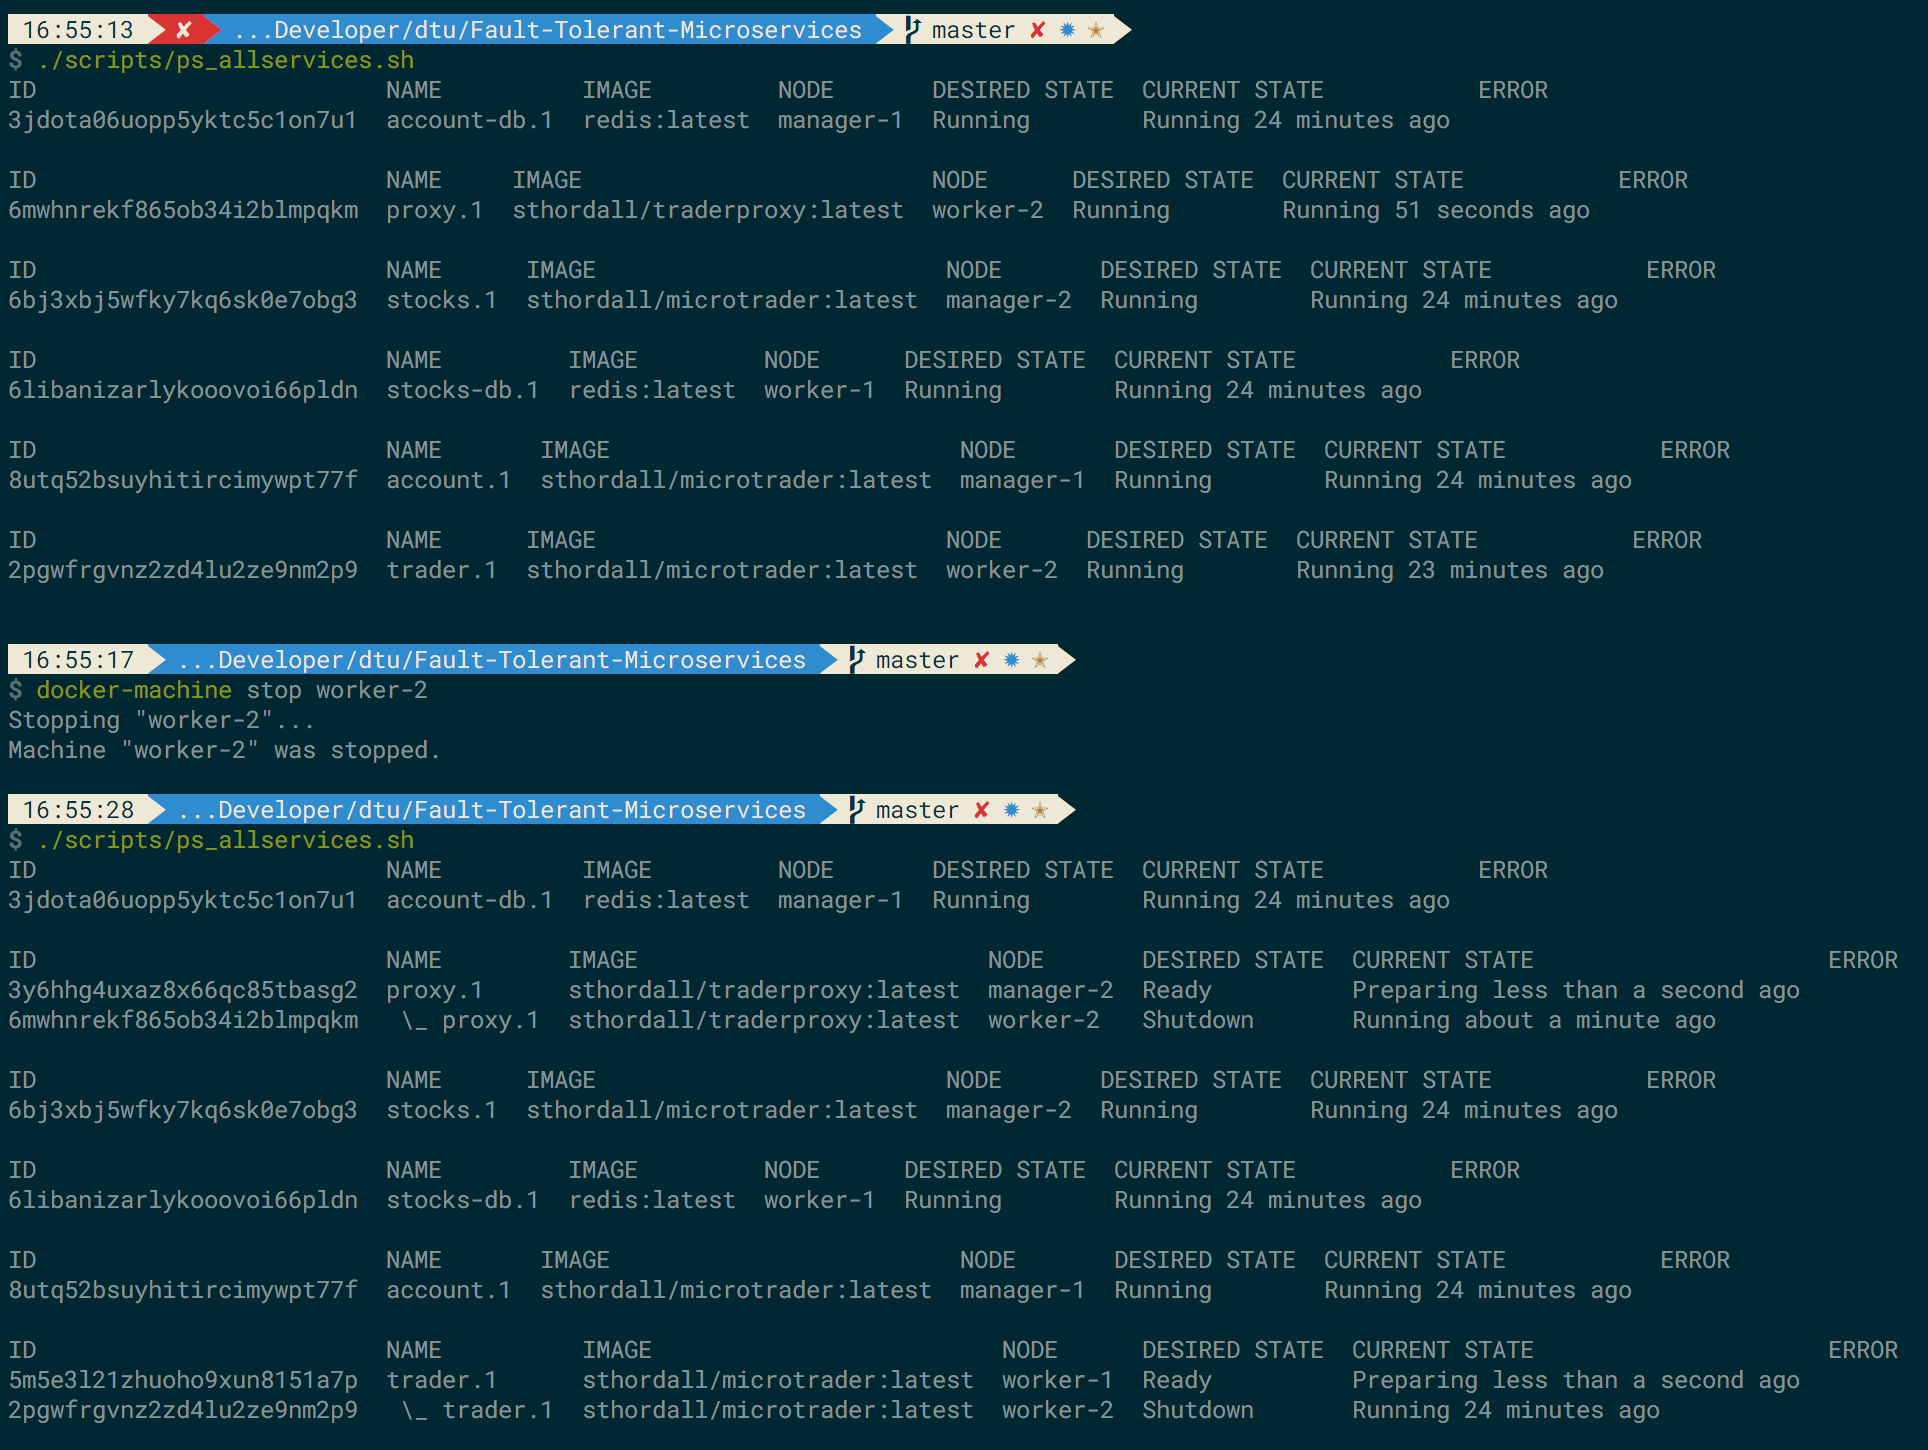
\includegraphics[width=0.9\textwidth]{../media/servicefailover.png} 
\caption{Demonstration of cluster node failover. The node 
	\texttt{worker\_2} is stopped, and the services previously running within it,
		are restarted on another node.}
\label{fig:servicefailover}
\end{figure}

\begin{figure}[H]
\centering
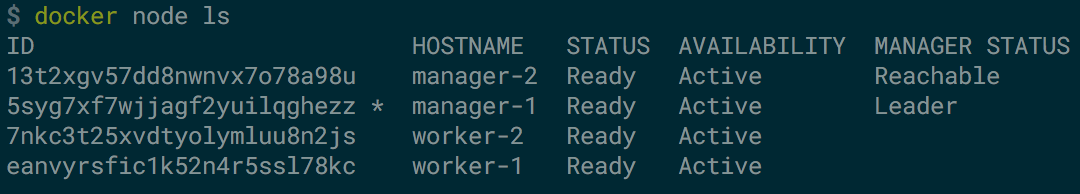
\includegraphics[width=0.49\textwidth]{../media/manager1leader.png} 
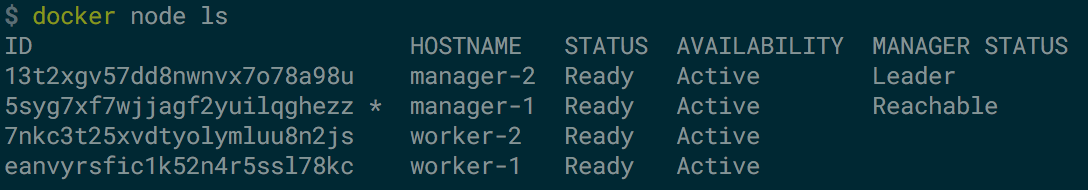
\includegraphics[width=0.49\textwidth]{../media/manager2leader.png} 
\caption{Output from running the \texttt{docker node ls} command, showing the nodes
		participating in the cluster and their status. The cluster is setup with
		two managers and two workers. If the \texttt{manager\_1} fails, \texttt{manager\_2} takes
		over. This involves restarting the services that ran within \texttt{manager\_1},
		across the other nodes. On the left \texttt{manager\_1} is leader, the
		VM with \texttt{manager\_1} was restarted, resulting in \texttt{manager\_2}
		becoming leader, seen on the right. }
\label{fig:manager1leader}
\end{figure}
